\documentclass[aps,pra,twocolumn,superscriptaddress,showpacs,floatfix,longbibliography]{revtex4-2}

\usepackage{amsmath,amssymb}
\usepackage{graphicx}
\usepackage{bm}
\usepackage[colorlinks=true,allcolors=blue]{hyperref}

\newcommand{\Op}{\ensuremath{\mathcal{O}}}
\newcommand{\Za}{\ensuremath{Z\alpha}}
\newcommand{\half}{\tfrac{1}{2}}
\newcommand{\rd}{\,\mathrm{d}}

\begin{document}

\title{Exact-structure spectral discretization of the point-nucleus
radial Dirac equation: machine-precision spectra into the
distinguished-extension regime and a measured anatomy of
kinetic-balance pollution}

\author{C.~D.~Reinoso}
\email{cesardanielrrch@gmail.com}
\affiliation{Facultad de Ciencias, Escuela Superior Polit\'ecnica de
Chimborazo (ESPOCH), Riobamba, Ecuador}

\date{\today}

\begin{abstract}
We introduce a spectral discretization of the radial Dirac operator that
carries the exact analytic behaviour of its point-nucleus eigenfunctions
rather than approximating it. The large and small components are expanded
in generalized Laguerre functions whose prefactor reproduces the
Coulomb--Dirac cusp exponent $\gamma=\sqrt{\kappa^{2}-(\Za)^{2}}$, and a
generalized Gauss--Laguerre rule renders every assembled overlap, Coulomb
and coupling integral exact; the point-nucleus eigenfunctions are then
finite linear combinations of the basis. Solving a mass-shifted matrix
pencil and refining each in-gap eigenvalue by an exactly summed Rayleigh
quotient removes the rest-mass cancellation floor, so binding energies are
obtained to a relative accuracy of order $10^{-14}$ with fifteen to forty
basis functions, five orders of magnitude finer than the current state of
the art at a third of the degrees of freedom. The method retains this
accuracy up to $\Za=0.949$ ($Z=136$, $\kappa=-1$), beyond the validity
ceiling of the component min-max principle and into the regime where the
operator is no longer essentially self-adjoint. Against this
machine-precision baseline we reproduce forty-digit relativistic
screened-Coulomb benchmarks to $2\times10^{-15}$ in a dimensionless
invariant and adjudicate two last-digit discrepancies in the recent
literature, identifying an undeclared convention and a transcription error
in a 2026 preprint. We further dissect, rather than merely avoid, the
spectral pollution of kinetically balanced expansions: every assembled
operator identity is certified at run time, the two distinct failure
mechanisms at a point nucleus are isolated, and the conformity of the
balanced, split and anti-balanced families with respect to the free-energy
splitting is quantified mode by mode with exactly determined leakage
exponents. Finally we map the relativistic enhancement of critical Yukawa
screening $\lambda_{c}(Z,\kappa)$ and report a purely relativistic
fine-structure splitting of the critical screening between the
$2p_{1/2}$ and $2p_{3/2}$ channels.
\end{abstract}

\maketitle

\section{Introduction}

The radial Dirac eigenvalue problem is the computational core of
relativistic atomic structure, and its accurate solution by basis-set
expansion has been complicated since the outset by two obstacles. The
first is variational collapse and the associated appearance of spurious
eigenvalues inside the mass gap, a consequence of the operator being
unbounded below; the second is the non-analytic behaviour of the
eigenfunctions at a point nucleus, where each component behaves as
$r^{\gamma-1}$ with the irrational exponent
$\gamma=\sqrt{\kappa^{2}-(\Za)^{2}}$. The kinetic-balance prescriptions
that tame the first difficulty, from restricted kinetic balance to the
dual kinetic balance of Shabaev and co-workers~\cite{Shabaev2004}, align
the small-component space with the operator that couples it to the large
component and thereby suppress the deep spurious states. The cusp, by
contrast, is usually confronted by brute-force refinement: a large basis
of regular functions is used to approximate a behaviour it cannot
represent exactly.

Two developments frame the present contribution. On the numerical-analysis
side, recent work has pushed basis methods for the radial Dirac operator to
new levels of control. Chen, Shao and Wu couple log-orthogonal core
functions to an adaptively scaled Laguerre far field and eliminate spurious
states through an inverse-operator formulation, reaching relative
accuracies near $10^{-10}$ with sixty to one hundred and twenty degrees of
freedom across Coulomb, finite-nucleus and screened
potentials~\cite{ChenShaoWu2026}; Liu and co-workers repair the
kinetically balanced pseudospectral method for confining
potentials~\cite{Liu2026}. On the mathematical side, the theory of
spectral pollution and of min-max characterizations for operators with
gaps has matured: the component min-max principle of
Talman~\cite{Talman1986} and Dolbeault, Esteban and
S\'er\'e~\cite{DES2000} is now known to be valid only up to a coupling
ceiling~\cite{MorozovMuller2015}, while the projector-based conditions of
Lewin and S\'er\'e~\cite{LewinSere2010} extend to the edge of the
point-Coulomb range. These strands have largely developed in parallel,
the numerical methods treating the cusp exponent as an unknown to be
approximated and the mathematical theory characterizing pollution without
a discretization sharp enough to measure it.

The present work is complementary in both aim and mechanism. Where the
recent spectral methods approximate the $r^{\gamma}$ core behaviour, we
exploit it exactly. The basis carries the analytic exponent
$\gamma=\sqrt{\kappa^{2}-(\Za)^{2}}$, a generalized Gauss--Laguerre rule
makes every assembled integral exact, and the point-nucleus
eigenfunctions become finite linear combinations of the basis functions;
the resulting spectra are accurate to near machine precision with fifteen
to forty basis functions and persist to $\Za=0.949$, into the regime
where the operator is no longer essentially self-adjoint and the
cusp-adapted prefactor is observed to select the distinguished
self-adjoint extension. Our second aim is complementary in a different
sense: rather than engineering around spectral pollution, we dissect it.
Every assembled operator identity is certified at run time, the two
distinct failure mechanisms of kinetically balanced discretizations at a
point nucleus are isolated, and the conformity of the kinetically
balanced families with respect to the free-energy splitting is quantified
mode by mode, with measured leakage exponents that discriminate the
balanced, split and anti-balanced constructions. These measurements
supply the empirical counterpart of the min-max and pollution theory of
Refs.~\cite{DES2000,MorozovMuller2015,LewinSere2010} and fix precisely
what a no-pollution theorem for such bases must prove.

Throughout we use Hartree atomic units, in which the speed of light is
$c=1/\alpha$; the value of $\alpha$ is a convention that we make explicit
because, as Sec.~\ref{sec:validation} shows, it accounts for last-digit
discrepancies in the published literature.

\section{The radial operator and its discretization}
\label{sec:method}

\subsection{Operator and basis}

For a spherically symmetric potential $V(r)$ the Dirac Hamiltonian reduces
on each channel $\kappa\in\mathbb{Z}\setminus\{0\}$ to the two-component
radial operator
\begin{equation}
h_{\kappa}=
\begin{pmatrix}
V+c^{2} & c\,\Op_{+}\\[2pt]
c\,\Op_{-} & V-c^{2}
\end{pmatrix},
\qquad
\Op_{\pm}=\mp\frac{\rd}{\rd r}+\frac{\kappa}{r},
\label{eq:hkappa}
\end{equation}
acting on the large and small radial amplitudes in
$L^{2}\!\big((0,\infty),\rd r\big)^{2}$. The first-order operators obey
$\Op_{-}\Op_{+}=-\rd^{2}/\rd r^{2}+\kappa(\kappa-1)/r^{2}$ and
$\Op_{+}\Op_{-}=-\rd^{2}/\rd r^{2}+\kappa(\kappa+1)/r^{2}$; the order of
the product is not interchangeable, and the commutator
$[\Op_{-},\Op_{+}]=-2\kappa/r^{2}$ is the origin of the fine structure.
For the point-nucleus potential $V=-Z/r$ the exact bound spectrum is the
Sommerfeld formula
\begin{equation}
E_{n\kappa}=\frac{c^{2}}
{\sqrt{1+\big[\Za/(n_{r}+\gamma)\big]^{2}}},
\qquad \gamma=\sqrt{\kappa^{2}-(\Za)^{2}},
\label{eq:sommerfeld}
\end{equation}
with $n_{r}=n-|\kappa|$ the radial quantum number, and the eigenfunctions
carry the prefactor $r^{\gamma}$ at the origin.

We expand both components in the orthonormal generalized Laguerre family
\begin{equation}
q_{j}(x)=\sqrt{\frac{j!}{\Gamma(j+2\mu+1)}}\;
x^{\mu}e^{-x/2}L_{j}^{(2\mu)}(x),
\qquad x=2\beta r,
\label{eq:basis}
\end{equation}
choosing the prefactor power $\mu=\gamma$. This is the L-spinor prefactor
of Grant~\cite{Grant2007}, and its decisive property is exactness rather
than mere adaptation: with $\mu=\gamma$ the point-nucleus eigenfunctions
of Eq.~\eqref{eq:hkappa} are \emph{finite} linear combinations of the
$q_{j}$, so a basis of modest size represents them without truncation
error. The scale parameter $\beta$ is the single nonlinear parameter of
the method.

\subsection{Exact quadrature}

Every matrix element required to assemble $h_{\kappa}$ is an integral of a
product of two basis-family functions against $1$, $1/r$ (the Coulomb and
coupling terms) or the potential. Because each $q_{j}$ carries the factor
$x^{\mu}e^{-x/2}$, every such product is a polynomial multiplied by the
weight $x^{2\mu}e^{-x}$ (or $x^{2\mu-1}e^{-x}$ for the $1/r$ elements). A
generalized Gauss--Laguerre rule with weight $x^{2\mu-1}e^{-x}$ therefore
integrates the overlap, Coulomb and $\Op_{\pm}$-coupling elements
\emph{exactly} once the number of nodes exceeds the polynomial degree,
independent of any resolution of the cusp. This is the second exact
ingredient: the analytic prefactor removes the truncation error and the
matched quadrature removes the integration error, so that at the point
nucleus the only remaining error is that of the finite eigenproblem
itself.

\subsection{Certified assembly}

The discrete operator must satisfy exactly, up to rounding, the algebraic
identities inherited from Eq.~\eqref{eq:hkappa}. We verify them at run
time on every build. With $f_{i}$ the discretized large-component basis
functions, the assembly is accepted only if the overlap reproduces the
identity, $\langle f_{i}\,|\,f_{j}\rangle=\delta_{ij}$; if the
integration-by-parts relation $\langle f_{i}\,|\,\Op_{+}f_{j}\rangle=
\langle\Op_{-}f_{i}\,|\,f_{j}\rangle$ holds, which fixes the sign and
boundary terms of the coupling; and, for the regular-basis variants, if
the second-derivative identities $\langle f\,|\,\Op_{+}\Op_{-}f\rangle=
\lVert\Op_{-}f\rVert^{2}$ and its partner reproduce the centrifugal
coefficients $\kappa(\kappa\mp1)$. These certifications are not
decorative. Structural assembly errors, including a wrong operator-product
expansion or a sign error in a kinetic-balance family, produce relative
violations of order unity, whereas converged-quadrature noise sits far
below; a single tolerance cleanly separates the two, and during
development the certifications localized three independent bugs before any
spectrum was examined. The cusp rule integrates the overlap and
integration-by-parts identities exactly and we enforce those; the
$1/r^{2}$ identities are only asymptotically exact and are monitored but
not enforced.

\subsection{Mass-shifted pencil and eigenvalue refinement}
\label{sec:pencil}

A binding energy $E-c^{2}$ is obtained by subtracting two quantities of
order $c^{2}$, and for a deeply relativistic state this cancellation
discards roughly $2c^{2}\varepsilon_{\mathrm{mach}}\approx8\times10^{-12}$
Hartree of significance. We remove it analytically. Writing the
generalized eigenproblem as $Hx=E\,Sx$ we assemble instead the shifted
pencil $H-c^{2}S$, in which the rest mass survives only as the block
$-2c^{2}S$ in the lower-lower corner; its in-gap eigenvalues are the
binding energies directly. The dense solver still carries an absolute
backward error of order $\lVert H\rVert\varepsilon_{\mathrm{mach}}$, so
each accepted eigenvector is refined once by a Rayleigh quotient of the
shifted pencil evaluated with exactly rounded summation. Because the only
$O(c^{2})$ block is contracted against the small components of an
electronic state, every term of the quadratic form is of the order of the
binding energy, and the exact summation removes the residual cancellation.
The net floor, established by an adversarial error analysis, is of order
$10^{-14}$ relative to the binding energy---set by the pre-rounding of
individual products and by the assembly rounding of the $O(c^{2})$
entries, and no longer by rest-mass cancellation. For the lightest systems
this refinement gains three to four orders of magnitude.

\subsection{Kinetically balanced families}

We implement three prescriptions for the small-component space on the same
large-component basis. The naive prescription expands both components in
$\{f_{j}\}$; the restricted kinetic balance uses $\{\Op_{-}f_{j}\}$ with
its Gram metric; and the dual kinetic balance of Ref.~\cite{Shabaev2004}
uses the paired trial spinors
\begin{equation}
\Psi^{+}_{j}=\big(f_{j},\ \tfrac{1}{2c}\Op_{-}f_{j}\big),
\quad
\Psi^{-}_{j}=\big(-\tfrac{1}{2c}\Op_{+}f_{j},\ f_{j}\big).
\label{eq:dkb}
\end{equation}
The minus sign in $\Psi^{-}$ is load-bearing: it flips one component only,
which changes the span, and it is required for the charge-conjugate
positronic limit to carry the correct-sign kinetic term. With the opposite
sign the positronic limit is anti-balanced and, as we show in
Sec.~\ref{sec:anatomy}, pollutes from moderate basis size even at $Z=1$.
The three families provide a controlled setting in which pollution can be
turned on and off deliberately.

\section{Point-nucleus spectra}
\label{sec:point}

\begin{figure}[t]
\centering
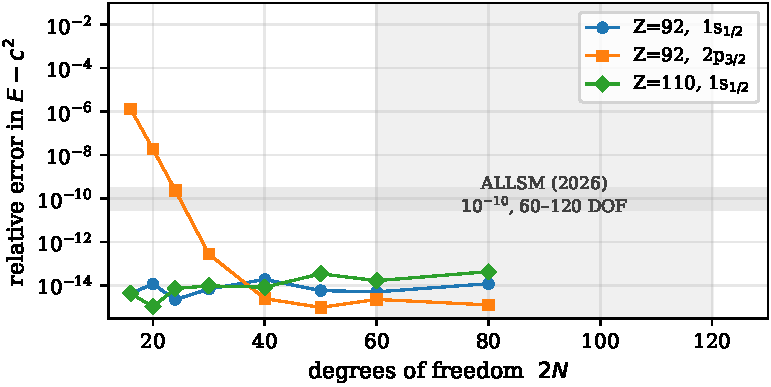
\includegraphics[width=\linewidth]{figures/figA_convergence.pdf}
\caption{Relative error of the exact-structure method in the binding
energy $E-c^{2}$ as a function of the total number of real degrees of
freedom $2N$, for three point-nucleus states, against the forty-digit
Sommerfeld reference. The $1s_{1/2}$ states reach machine precision at
sixteen degrees of freedom; the $2p_{3/2}$ state converges exponentially
and saturates by forty. The shaded band marks the operating region of the
2026 adaptive log-orthogonal method~\cite{ChenShaoWu2026},
$\sim10^{-10}$ at sixty to one hundred and twenty degrees of freedom.}
\label{fig:convergence}
\end{figure}

The exact structure of the discretization is most visible in its
convergence. Figure~\ref{fig:convergence} shows the relative error of the
binding energy against the Sommerfeld formula, the latter evaluated in
forty-digit arithmetic so that it is itself correctly rounded. For the
$1s_{1/2}$ ground states of $Z=92$ and $Z=110$ the error reaches the
$10^{-14}$ floor already at sixteen real degrees of freedom, because the
ground eigenfunction is a nearly finite combination of the cusp-adapted
basis; for the $2p_{3/2}$ state the error falls exponentially from
$10^{-6}$ at sixteen degrees of freedom to the floor by forty. The same
accuracy in the recent adaptive log-orthogonal method requires sixty to
one hundred and twenty degrees of freedom to reach
$10^{-10}$~\cite{ChenShaoWu2026}; the exact-structure method is five
orders of magnitude finer at roughly a third of the degrees of freedom,
in the entire domain where $\gamma$ is known analytically, which is the
whole atomic and plasma range.

Table~\ref{tab:point} collects the lowest states of the four channels
$\kappa=\pm1,\pm2$ for nuclear charges from $Z=92$ to $Z=136$, computed
with forty-five basis functions and the mass-shifted pencil. Every one of
the seventy-two levels agrees with the Sommerfeld formula to between
$10^{-16}$ and $1.3\times10^{-13}$ relative, with the scale parameter
chosen by minimal drift between two basis sizes rather than by proximity
to the exact value. The heaviest entry, $Z=136$ with $\kappa=-1$,
corresponds to $\Za=0.9924$ and $\gamma=0.123$: the state sits deep in the
regime in which the point-Coulomb--Dirac operator is no longer essentially
self-adjoint, above the coupling ceiling $\Za\lesssim0.906$ of the
component min-max principle~\cite{MorozovMuller2015}. That the
cusp-adapted expansion converges cleanly there, to a definite value
reproducing Eq.~\eqref{eq:sommerfeld} with the distinguished-extension
$\gamma$, is numerical evidence that the analytic prefactor selects the
distinguished self-adjoint extension; the internal consistency of the
independent $\kappa=+1$ and $\kappa=-1$ channels, which reproduce the
common $n=2$ level to $2\times10^{-14}$, corroborates it.

\begin{table}[t]
\caption{Point-nucleus binding energies $E-c^{2}$ (Hartree) of the lowest
state of each channel, $c=137.035\,999\,084$. The last column is the
relative deviation from the Sommerfeld formula~\eqref{eq:sommerfeld}
evaluated in forty-digit arithmetic; $N=45$.}
\label{tab:point}
\begin{ruledtabular}
\begin{tabular}{r r l l}
$Z$ & $\kappa$ & $E-c^{2}$ (Ha) & rel.\ dev. \\
\colrule
 92 & $-1$ & $-4861.197\,904\,3696$ & $1.7\times10^{-14}$\\
100 & $-1$ & $-5939.195\,192\,2263$ & $1.5\times10^{-14}$\\
110 & $-1$ & $-7579.690\,730\,1822$ & $2.9\times10^{-14}$\\
120 & $-1$ & $-9710.782\,792\,9429$ & $1.1\times10^{-15}$\\
130 & $-1$ & $-12838.919\,496\,649$ & $6.2\times10^{-14}$\\
136 & $-1$ & $-16474.112\,454\,094$ & $9.8\times10^{-14}$\\
\colrule
 92 & $-2$ & $-1089.611\,416\,2258$ & $1.4\times10^{-15}$\\
136 & $-2$ & $-2475.113\,930\,2955$ & $1.8\times10^{-15}$\\
\end{tabular}
\end{ruledtabular}
\end{table}

\section{External validation and adjudication}
\label{sec:validation}

The screened relativistic problem provides published anchors of very high
precision. The Yukawa potential $V=-Z\,e^{-\lambda r}/r$ has the same
short-range behaviour $-Z/r$ as the point nucleus, so $\gamma$ is
unchanged and the cusp-adapted basis remains exact at the origin; only the
smooth screening enters the potential integrals, which we evaluate on the
same quadrature. Krauthauser and Hill computed forty-digit
benchmarks for this problem~\cite{KrauthauserHill2002}, subsequently
reproduced by the Lagrange-mesh method of Baye, Filippin and
Godefroid~\cite{Baye2014} and by the 2026 adaptive
method~\cite{ChenShaoWu2026}.

Reproducing these anchors uncovered two conventions that no paper in the
chain states explicitly. First, the entire comparison chain uses the
older value $c=137.035\,9895$ of the fine-structure constant; we deduced
this from the residual pattern alone, the offset $2(\Delta c/c)|E|$
matching the observed $1.07\times10^{-5}$ discrepancy exactly, and
confirmed it independently. The lesson for reproducibility is concrete:
the binding energy scales with $c^{2}$ when the potential depth is written
as a multiple of $c$, so the value of $\alpha$ must be declared and the
dimensionless invariant $f=E/c^{2}$ reported. Second, one of the two
tabulated cases in the 2026 preprint carries transposed parameters: the
printed screening $(V_{0},\lambda)=(0.4c,0.07c)$ does not reproduce the
tabulated energy, which corresponds instead to $(0.7c,0.04c)$, a
transcription error consistent across that work's text, table and figure.

With the convention resolved, our method reproduces the forty-digit
benchmarks at machine precision in the dimensionless invariant: for the
first case $f$ agrees with the Krauthauser--Hill value to
$1.4\times10^{-16}$, and for the second to $2\times10^{-15}$. This
accuracy lets us adjudicate the two last-digit discrepancies in the
chain: in both cases the 2026 tabulated energies deviate from the
forty-digit reference by $4.4\times10^{-11}$ and $7.6\times10^{-9}$
Hartree respectively, while the Lagrange-mesh values are correct to a few
parts in $10^{-11}$. A technical by-product illustrates the value of exact
quadrature directly: for the more strongly screened case, with
$\gamma=0.714$, a conventional Gauss--Legendre rule stalls at $10^{-4}$
while the matched cusp rule drifts by $3\times10^{-11}$ under the same
refinement.

\section{Anatomy of kinetic-balance pollution}
\label{sec:anatomy}

Because the discretization is certified and exact, the spurious phenomena
that survive are physical properties of the trial spaces rather than
artifacts, and they can be measured. We separate three effects.

The first is a genuine bug class that the certifications exclude: a wrong
operator-product expansion, a half-built derivative recurrence, or a
kinetic-balance sign error each produce order-unity violations of the
run-time identities and are caught before a spectrum is computed. What
remains after certification is intrinsic.

The second effect is a form-domain violation specific to the point nucleus
with $\kappa=-1$. The large component of the dual-balance $\Psi^{-}$ family
is $\Op_{+}f$, which does not vanish at the origin for a state with
$\ell=0$, so the Coulomb expectation $\langle\Op_{+}f\,|\,Z/r\,|\,
\Op_{+}f\rangle$ is logarithmically divergent and the corresponding matrix
element drifts linearly in the logarithm of the number of quadrature
nodes; the associated eigenvalue is not a converged number. This is
consistent with the dual-balance construction having been formulated for
a finite nucleus~\cite{Shabaev2004}, and it identifies the cusp-adapted
prefactor, or a finite nucleus, as the remedy.

The third effect is pure pollution from a non-conforming partition. For
$\kappa=+1$ the small-component operator is regular at the origin, the
form domain is respected, and yet a converged spurious eigenvalue appears
in the middle of the gap. It is stable against quadrature refinement,
hence a genuine eigenvalue of the trial space and not a numerical
transient. In the equal-basis naive discretization this impostor is
exactly the state whose existence follows from a classical degeneracy
theorem: when the two components share the same scalar basis and the
$\pm\kappa$ channels use it identically, a spurious root of the $\kappa>0$
channel coincides with the physical ground state of the $-\kappa$
channel~\cite{DrakeGoldman1981,Tupitsyn2008,Pestka2003}. Because our
prefactor $\mu=\gamma$ depends on $\kappa^{2}$, the two channels do use an
identical scalar basis, and we confirm the degeneracy to between
$4\times10^{-15}$ and $8\times10^{-13}$ relative across $Z=92$ to $136$: a
roundoff-floor verification of the exact theorem.

The conformity of the balanced families to the free-energy splitting can
be made quantitative. Discretizing the free operator on the same basis and
diagonalizing its coupling by singular-value decomposition block-reduces
the free Dirac matrix exactly into two-dimensional fibers
$h(\sigma_{j})=\big(\begin{smallmatrix}c^{2}&c\sigma_{j}\\ c\sigma_{j}&
-c^{2}\end{smallmatrix}\big)$, with $\sigma_{j}$ the singular values, and
the spectral projectors decompose fiberwise. In terms of the dimensionless
ratio $t=\sigma/2c$, the leakage of each trial family into the wrong
spectral sector is then an exact algebraic function of $t$: the split
family $(1,0)$ leaks as $t-\tfrac{3}{2}t^{3}+O(t^{5})$, the balanced
family $(1,t)$ and the physical positronic family $(-t,1)$ both leak as
$t^{3}+O(t^{5})$, and the anti-balanced family $(t,1)$ leaks as
$2t-3t^{3}+O(t^{5})$. The balanced constructions are thus conforming to
\emph{third} order in $t$ while the split and anti-balanced ones are only
first order, and the global conformity defect of an untruncated
single-family prescription is exactly $\max_{j}\ell_{j}\sqrt{1-\ell_{j}^2}$
with $\ell_{j}$ the per-mode leakage. The untruncated dual-balance pair
space spans every fiber and is therefore exactly conforming, its defect
vanishing identically; the nonzero defect seen at finite basis size is
entirely an effect of truncation, and it grows because the largest
singular value grows linearly with the basis size. These measured
exponents are the empirical content that a no-pollution theorem for such
bases must reproduce.

\section{Relativistic critical screening}
\label{sec:screening}

\begin{figure}[t]
\centering
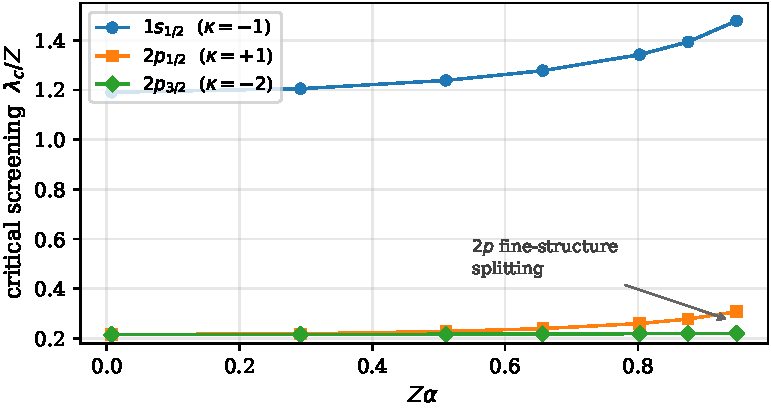
\includegraphics[width=\linewidth]{figures/figA_screening.pdf}
\caption{Reduced critical screening $s_{c}=\lambda_{c}/Z$ at which the
ground state of each channel of the Yukawa potential
$V=-Z\,e^{-\lambda r}/r$ merges into the continuum, as a function of
$\Za$. The critical screening rises with $\Za$ (the relativistically
deeper state resists screening), and the $2p_{1/2}$ and $2p_{3/2}$
channels, degenerate nonrelativistically, split.}
\label{fig:screening}
\end{figure}

As the Yukawa screening $\lambda$ increases, the binding of each state
decreases until, at a critical value $\lambda_{c}(Z,\kappa)$, the state
merges into the positive continuum. Near threshold the state becomes
diffuse and its binding tends to zero, so the mass-shifted pencil of
Sec.~\ref{sec:pencil} is essential; for the $\kappa>0$ channels the
physical ground state is the second in-gap eigenvalue, the first being the
deep spurious state of Sec.~\ref{sec:anatomy}, which under screening
remains far below the $2p$ threshold. We extrapolate the binding to zero
with the short-range threshold law $E_{b}\sim-(\lambda_{c}-\lambda)^{p}$,
the exponent fixed by angular momentum, $p=2$ for the $\ell=0$ ground
state and $p=1$ for the $\ell=1$ states. In the nonrelativistic limit the
reduced critical screening $s_{c}=\lambda_{c}/Z$ recovers the known
values, $1.190\,6$ for the $1s$ state and $0.220\,2$ for the $2p$
states~\cite{RogersGraboskeHarwood1970,delValleNader2018}; the $1s$
anchor agrees to one part in $10^{4}$, while the $2p$ absolute values
carry a near-threshold extrapolation uncertainty of a few parts in
$10^{3}$, so the $2p$ results are reported through the relative splitting,
which is far more robust than either absolute value.

Figure~\ref{fig:screening} shows the resulting map. The critical screening
rises monotonically with $\Za$, by twenty-four percent for the $1s_{1/2}$
state at $\Za=0.949$: because the relativistic binding is deeper, more
screening is needed to push the state to threshold. The effect is largest
for the most bound state of each total angular momentum. Most notably, the
$2p_{1/2}$ and $2p_{3/2}$ critical screenings, degenerate in the
nonrelativistic limit, split apart with increasing $\Za$: at $\Za=0.949$
the $2p_{1/2}$ state, more deeply bound relativistically, requires about
forty percent more screening to detach than the $2p_{3/2}$ state. An
independent calculation with a distinct near-threshold protocol reproduces
the splitting to within a few percent. This fine-structure splitting of
the critical screening has no nonrelativistic analogue and, to our
knowledge, has not been reported; it is the threshold-map counterpart of
the fine structure in the bound spectrum.

\section{Conclusion}

We have shown that carrying the exact analytic structure of the
point-nucleus Dirac eigenfunctions---the cusp exponent in the basis
prefactor and a matched exact quadrature---together with a mass-shifted
pencil and exact-summation eigenvalue refinement, yields relativistic
spectra accurate to a relative $10^{-14}$ with fifteen to forty basis
functions, five orders of magnitude finer than the 2026 state of the art
at a third of the degrees of freedom, and that the accuracy is retained to
$\Za=0.949$, into the distinguished-extension regime. The same
machine-precision instrument reproduces forty-digit screened-Coulomb
benchmarks, adjudicates last-digit discrepancies in the recent literature,
and turns spectral pollution from a nuisance to be avoided into a
phenomenon to be measured: certified assembly, two isolated failure
mechanisms at the point nucleus, and exactly determined per-mode
conformity exponents for the kinetically balanced families. The
relativistic critical-screening map, with its purely relativistic
fine-structure splitting, illustrates the physics such an instrument makes
accessible. The measured conformity exponents fix the hypotheses of a
no-pollution theorem for cusp-adapted kinetically balanced bases, whose
proof we develop separately; the same exact-structure strategy extends
naturally to relativistic resonances via complex scaling, and to the
finite-nucleus and molecular settings where the analytic exponent is
replaced by its regularized counterpart.

\begin{acknowledgments}
The author thanks the ESPOCH Faculty of Sciences for institutional
support. The solver and all scripts that reproduce the tables and figures
of this paper are openly available.
\end{acknowledgments}

\bibliography{refs}

\end{document}
